% Permission is granted to copy, distribute and/or modify this document
% under the terms of the GNU Free Documentation License, Version 1.3
% or any later version published by the Free Software Foundation;
% with no Invariant Sections, no Front-Cover Texts, and no Back-Cover Texts.
% A copy of the license is included in the section entitled "GNU
% Free Documentation License".
%
% Written (C) 2012-2013 Heiko Strathmann
% Written (C) 2012 Sergey Lisitsyn

\documentclass{shogun_tutorial}
\tolerance=2000
% Permission is granted to copy, distribute and/or modify this document
% under the terms of the GNU Free Documentation License, Version 1.3
% or any later version published by the Free Software Foundation;
% with no Invariant Sections, no Front-Cover Texts, and no Back-Cover Texts.
% A copy of the license is included in the section entitled "GNU
% Free Documentation License".
%
% Written (C) 2012 Heiko Strathmann

\DeclareMathOperator{\mmd}{MMD}
\DeclareMathOperator{\tr}{tr}
\DeclareMathOperator{\var}{var}
\DeclareMathOperator{\cov}{cov}
\DeclareMathOperator{\diag}{diag}

\title{SHOGUN-tutorial}
\date{\today}
\author
{
Sergey Lisitsyn \and 
Heiko Strathmann\and 
Chiyuan Zhang \and 
}

\begin{document}
	\maketitle
	Copyright \copyright{}  2012-2013 Shogun developers.
    Permission is granted to copy, distribute and/or modify this document
    under the terms of the GNU Free Documentation License, Version 1.3
    or any later version published by the Free Software Foundation;
    with no Invariant Sections, no Front-Cover Texts, and no Back-Cover Texts.
    A copy of the license is included in the section entitled ``GNU
    Free Documentation License''.
    
    
	\tableofcontents
	\listoftodos
	\part{Essentials}
	\chapter{Learning}

In this part we outline essentials of machine learning.

\section{Learning is a search process}

\section{Empirical risk minimization (ERM) principle}

\section{Structural risk minimization (SRM) principle}

\section{Linear models}

\section{Supervised learning}

\subsection{Classification}

\subsection{Regression}

\section{Unsupervised learning}

\subsection{Clustering}

\subsection{Dimensionality reduction}

\section{Transfer learning}

\subsection{Multitask learning}

\subsection{Domain adaptation}

	
	\part{Objects in \shogun{}}
	% Permission is granted to copy, distribute and/or modify this document
% under the terms of the GNU Free Documentation License, Version 1.3
% or any later version published by the Free Software Foundation;
% with no Invariant Sections, no Front-Cover Texts, and no Back-Cover Texts.
% A copy of the license is included in the section entitled "GNU
% Free Documentation License".
%
% Written (C) 2012 Heiko Strathmann

\chapter{Kernels}

In this chapter, we describe how kernels are represented in \shogun{} and provide a list of implemented ones.

	% Permission is granted to copy, distribute and/or modify this document
% under the terms of the GNU Free Documentation License, Version 1.3
% or any later version published by the Free Software Foundation;
% with no Invariant Sections, no Front-Cover Texts, and no Back-Cover Texts.
% A copy of the license is included in the section entitled "GNU
% Free Documentation License".
%
% Written (C) 2012 Heiko Strathmann

\chapter{Data Representations -- Features}
\label{chp:shogun_objects-features}

In this chapter, we describe how data or features are represented in \shogun{} and provide a list of implemented ones.
\todo{Document features framework}

\section{Dense Features}
\label{sec:shogun_objects-features-dense}
\todo{Document dense features}


\section{Streaming Features}
\label{sec:shogun_objects-features-streaming}
\todo{Document streaming features. H.S.}

	
	\part{Algorithms}
	
	% Permission is granted to copy, distribute and/or modify this document
% under the terms of the GNU Free Documentation License, Version 1.3
% or any later version published by the Free Software Foundation;
% with no Invariant Sections, no Front-Cover Texts, and no Back-Cover Texts.
% A copy of the license is included in the section entitled "GNU
% Free Documentation License".
%
% Written (C) 2012 Chiyuan Zhang

\chapter{Multiclass learning}

In this chapter we describe multiclass learning algorithms available in the 
\shogun{} toolbox.  Multiclass learning refers to the problem with the output 
space $\mathcal{Y}=\{1,\ldots,K\}$\footnote{Note while we describe the class 
	numbers as from $1$ to $K$, the multiclass machines in \shogun{} expect 
	the examples to be labeled with $0,\ldots,K-1$.}, where $K>2$.  Most of 
real world machine learning classification problems are naturally multiclass.   
Typical examples include document categorization, image classification, 
hand-written digit recognition, etc.  

Generally, no assumption of any specific structure for the set $\mathcal{Y}$
are made in multiclass learning.  When priori knowledge are available for a
rich structure of $\mathcal{Y}$, \emph{structured-output learning} algorithms
are usually used instead.

Many algorithms, like K-Nearest Neighbors and Naive Bayes, handle both 
multiclass problems and binary problems naturally (and in an uniform way). 
Those are described in section~\ref{sec:multiclass-natural}. 
Section~\ref{sec:multiclass-reduction} describes reduction from multiclass 
problems into binary problems. Tree-styled classifiers are described in 
section~\ref{sec:multiclass-tree}.

Several standard datasets are used by examples in this chapter. We summarize
them in Table~\ref{tab:multiclass-dataset}. All of those datasets can be found
in \url{http://mldata.org}.

\begin{table}[t]\centering
	\begin{tabular}{ccccc}
		\toprule
		Name & \# Classes & \# Samples & \# Attributes & Remarks \\
		\midrule
		USPS & 10         & 9298       & 256           & Hand-written Digits \\
		\bottomrule
	\end{tabular}
	\caption{Standard datasets for multiclass learning used in examples.}
	\label{tab:multiclass-dataset}
\end{table}

\section{Natural Multiclass Algorithms}
\label{sec:multiclass-natural}

\subsection{K-Nearest Neighbors}
\emph{K-Nearest Neighbors} (KNN) is a very simple and effective algorithm. The 
learning step actually does nothing but memorizing all the training points and 
the associated labels. The prediction is carried out by finding the $K$ 
nearest neighbors of the query point, and then voting.  Here $K$ is a 
hyper-parameter for the algorithm. Smaller $K$ gives the model low bias but 
high variance; while larger $K$ gives low variance but high bias.

KNN has attracted focus from both industrial and academia ever since its
conception. It is easy to implement, and can handle almost arbitrarily complex
problem by adjusting one single parameter $K$. Besides, it also has many nice
theoretical properties \citep{ProbTheoryofPR}.

In \shogun, you can use \shogunclass{CKNN} to perform KNN learning. To
construct a KNN machine, you must choose the hyper-parameter $K$ and a distance
function. Usually, we simply use the \shogunclass{CEuclideanDistance}, but in
general, any subclass of \shogunclass{CDistance} can be used. For
demonstration, we select a random subset of 1000 samples from USPS, and run
2-fold cross validation of KNN on it with varying $K$. The accuracy is shown in
Fig.~\ref{fig:mc-knn-acc}.

In \shogun{}, you can also use \emph{Cover Tree} \citep{CoverTree} to speed up
the nearest neighbor searching process in KNN. Just call \Verb|set_use_covertree| on
the KNN machine to enable or disable this feature. The prediction time
comparison for this experiment with and without Cover Tree are shown in
Fig.~\ref{fig:mc-knn-time}.

\begin{figure}\centering
	\begin{subfigure}{.48\textwidth}
		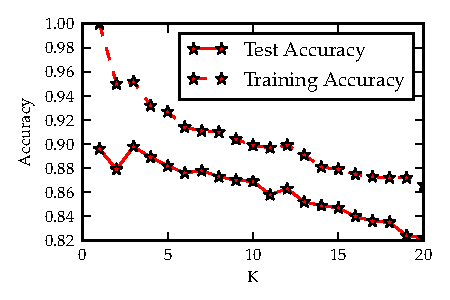
\includegraphics{fig/multiclass/knn-accuracy}
		\caption{KNN classification accuracy on USPS.}
		\label{fig:mc-knn-acc}
	\end{subfigure}
	~
	\begin{subfigure}{.48\textwidth}
		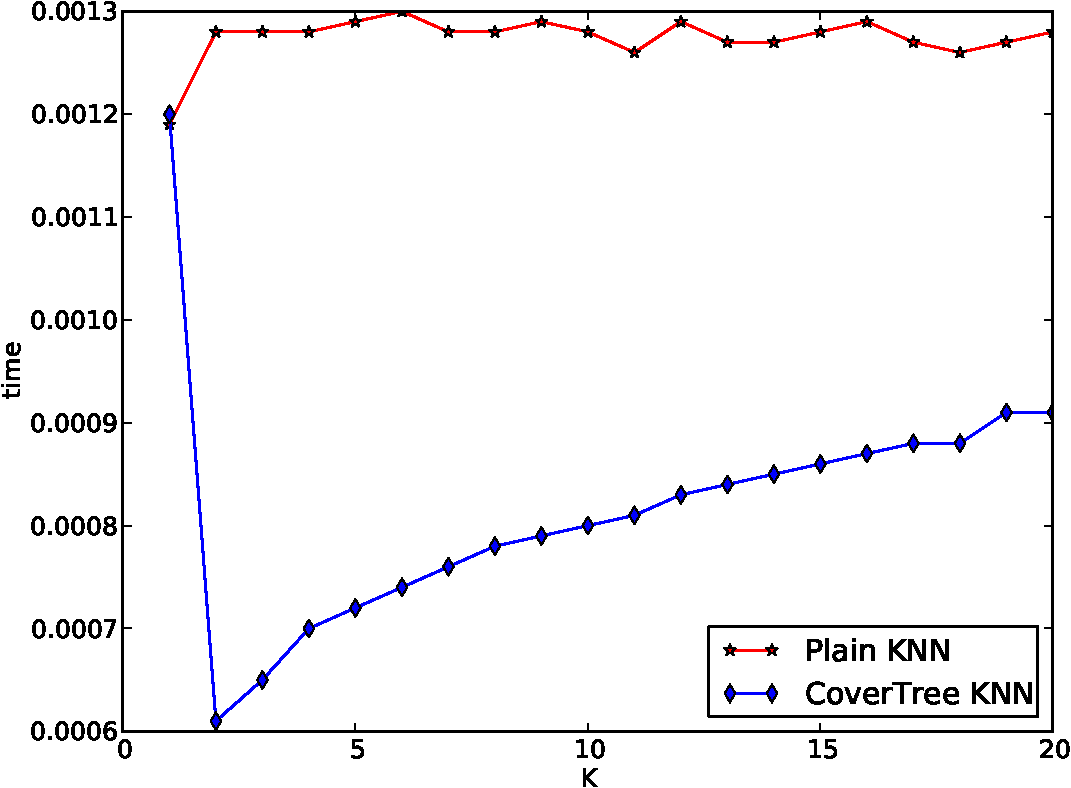
\includegraphics{fig/multiclass/knn-time}
		\caption{Prediction time (per example) with and without CoverTree.}
		\label{fig:mc-knn-time}
	\end{subfigure}
	\caption{KNN classification on a random subset (1000 samples) of USPS.}
\end{figure}

Although simple and elegant, KNN is generally very resource costly. Because all
the training samples are to be memorized literally, the memory cost of KNN
``learning'' becomes prohibitive when the dataset is huge. Even though the
memory is big enough to hold all the data, the prediction will be slow, since
the distances between the query point and all the training points need to be
computed and ranked. The situation becomes worse if in addition the data
samples are all very high-dimensional.

\subsection{Naive Bayes}
\emph{Naive Bayes} is a simple and fast algorithm for multiclass learning.
Formally, it predict the class by computing the posterior probability of each
class $k$ after observing the input $x$:

\[
	P\left( Y=k | X = x \right) = \frac{P(X=x|Y=k)P(Y=k)}{P(X=x)}
\]

The prediction is then made by

\[
	y = \argmax_{k\in\{1,\ldots,K\}} P(Y=k|X=x)
\]

Since $P(X=x)$ is a constant factor for all $P(Y=k|X=x)$, $k=1,\ldots,K$, there
is no need to compute it.

In \shogun{}, \shogunclass{CGaussianNaiveBayes} implements the Naive Bayes
algorithm. It is prefixed with ``Gaussian'' because the probability model for
$P(X=x|Y=k)$ for each $k$ is taken to be a multi-variate Gaussian distribution.
Furthermore, each dimension of the feature vector $X$ is assumed to be
independent. The ``Naive'' independence assumption enables us the learn the
model by estimating the parameters for each feature dimension independently,
thus the whole learning algorithm runs very quickly. And this is also the 
reason for its name. However, this assumption can be very restrictive. In
Fig.~\ref{fig:mc-gnb-fail}, we show a simple 2D example. There are 3 linearly
separable classes. The scattered points are training samples with colors
indicating their labels. The filled area indicate the hypothesis learned by
the \shogunclass{CGaussianNaiveBayes}. The training samples are actually
generated from three Gaussian distributions. But since the covariance for those
Gaussian distributions are not diagonal (i.e. there are ``rotations''), the GNB
algorithm cannot handle them properly.

\begin{figure}
    \centering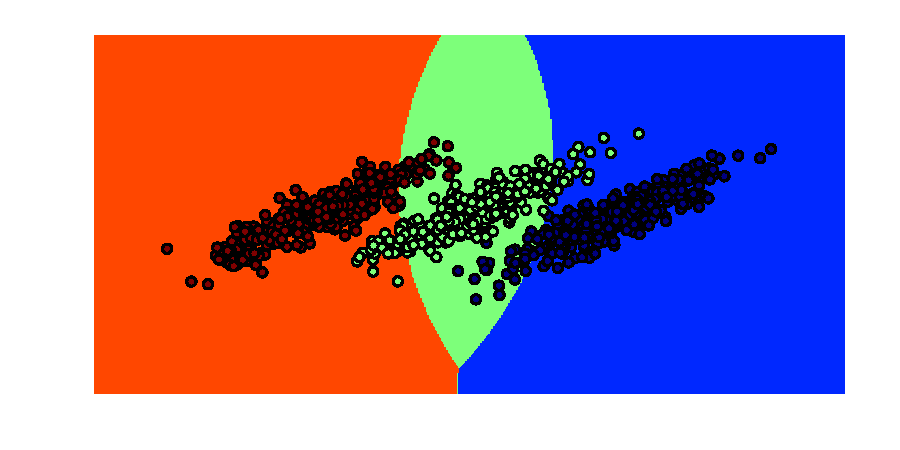
\includegraphics{fig/multiclass/gnb-fail-case}
    \caption{Gaussian Naive Bayes fails to learn on a simple 2D example with 3
    linearly separable classes.}
    \label{fig:mc-gnb-fail}
\end{figure}

Although the independent assumption is usually considered to be too optimistic 
in reality, Naive Bayes sometimes works very well in some applications. For 
example, in email spam filtering, Naive Bayes\footnote{More specifically, the 
    discrete Naive Bayes is generally used in this scenario. The main 
    difference with Gaussian Naive Bayes is that a tabular instead of a 
    parametric Gaussian distribution is used to describe the likelihood 
    $P(X=x|K=k)$.} is a very popular and widely used method.

This algorithm is closely related to the \emph{Gaussian Mixture Model} (GMM) learning
algorithm. However, while GMM is an unsupervised learning algorithm, Gaussian
Naive Bayes is supervised learning. It uses the training labels to directly
estimate the Gaussian parameters for each class, thus avoids the iterative
\emph{Expectation Maximization} procedures in GMM.

The merit of GNB is that both training and predicting are very fast, and it has
no hyper-parameters.

\subsection{Logistic Regression}

Although named logistic \emph{regression}, it is actually a classification
algorithm. Similar to \emph{Naive Bayes}, logistic regression computes the
posterior $P(Y=k|X=x)$ and makes prediction by

\[
    y = \argmax_{k\in\{1,\ldots,K\}} P(Y=k|X=x)
\]

However, Naive Bayes is a \emph{generative model}, in which the distribution of
the input variable $X$ is also modeled (by a Gaussian distribution in this
case). But logistic regression is a \emph{discriminative model}, which doesn't
care about the distribution of $X$, and models the posterior directly.
Actually, the two algorithms are a \emph{generative-discriminative pair}
\citep{DBLP:conf/nips/NgJW01}.

To be specific, logistic regression uses \emph{linear} functions in $X$ to model the
posterior probabilities:

\begin{eqnarray}
    \log\frac{P(Y=1|X=x)}{P(Y=K|X=x)} &=& \beta_{10} + \beta_1^Tx \\
    \log\frac{P(Y=2|X=x)}{P(Y=K|X=x)} &=& \beta_{20} + \beta_2^Tx \\
    &\vdots& \nonumber\\
    \log\frac{P(Y=K-1|X=x)}{P(Y=K|X=x)} &=& \beta_{(K-1)0} + \beta_{K-1}^Tx
\end{eqnarray}

The training of a logistic regression model is carried out via \emph{maximum
    likelihood estimation} of the parameters
$\boldsymbol\beta = \{\beta_{10},\beta_1^T,\ldots,\beta_{(K-1)0},\beta_{K-1}^T\}$. There is no
closed form solution for the estimated parameters.

There is not independent implementation of logistic regression in \shogun{}, 
but the \shogunclass{CLibLinear} becomes a logistic regression model when
constructed with the argument \Verb|L2R_LR|. This model also include a
regularization term of the $\ell_2$-norm of $\boldsymbol\beta$. If sparsity in
$\boldsymbol\beta$ is needed, one can also use \Verb|L1R_LR|, which replaces
the $\ell_2$-norm regularizer with a $\ell_1$-norm regularizer.

Unfortunately, the logistic regression in \shogun{} does not support multiclass
problem yet.

\section{Reduction to Binary Problems}
\label{sec:multiclass-reduction}

Since binary classification problems are one of the most thoroughly studied
problems in machine learning, it is very appealing to consider reducing
multiclass problems to binary ones. Then many advanced learning and
optimization techniques as well as generalization bound analysis for binary
classification can be utilized.

In \shogun{}, the strategies of reducing a multiclass problem to binary
classification problems are described by an instance of
\shogunclass{CMulticlassStrategy}. A multiclass strategy describes
\begin{enumerate}
\item How to train the multiclass machine as a number of binary machines?
	\begin{itemize}
		\item How many binary machines are needed?
		\item For each binary machine, what subset of the training samples are
			used, and how are they colored\footnote{In multiclass problems, we
				use \emph{coloring} to refer partitioning the classes into two
				groups: $+1$ and $-1$, or black and white, or any other meaningful
				names.}?
	\end{itemize}
\item How to combine the prediction results of binary machines into the final
	multiclass prediction?
\end{enumerate}

The user can derive from the virtual class \shogunclass{CMulticlassStrategy} to
implement a customized multiclass strategy. But usually the built-in strategies
are enough for general problems. We will describe the built-in \emph{One-vs-Rest},
\emph{One-vs-One} and \emph{Error-Correcting Output Codes} strategies in the
following subsections.

The basic routine to use a multiclass machine with reduction to binary problems
in shogun is to create a generic multiclass machine and then assign a particular
multiclass strategy and a base binary machine.

\subsection{One-vs-Rest and One-vs-One}

The \emph{One-vs-Rest} strategy is implemented in
\shogunclass{CMulticlassOneVsRestStrategy}. As indicated by the name, this
strategy reduce a $K$-class problem to $K$ binary sub-problems. For the $k$-th
problem, where $k\in\{1,\ldots,K\}$, the samples from class $k$ are colored as
$+1$, and the samples from other classes are colored as $-1$. The multiclass
prediction is given as

\[
	f(x) = \argmax_{k\in\{1,\ldots,K\}} f_k(x)
\]
where $f_k(x)$ is the prediction of the $k$-th binary machines.

The One-vs-Rest strategy is easy to implement yet produces the good performance
in many cases. One interesting paper \citep{OneVsRestDefense} shows that the
One-vs-Rest strategy can be

\begin{quote}
	\emph{as accurate as any other approach, assuming that the underlying binary
classifiers are well-tuned regularized classifiers such as support vector
machines.}
\end{quote}

Implemented in \shogunclass{CMulticlassOneVsOneStrategy}, the 
\emph{One-vs-One} strategy \citep{OneVsOne} is another simple and intuitive 
strategy: it basically produces one binary problem for each pair of classes.  
So there will be $\binom{K}{2}$ binary problems. At prediction time, the 
output of every binary classifiers are collected to do voting for the $K$ 
classes. The class with the highest vote becomes the final prediction.

Compared with the One-vs-Rest strategy, the One-vs-One strategy is usually more
costly to train and evaluate because more binary machines are used.

In the following, we demonstrate how to use \shogun{}'s One-vs-Rest and 
One-vs-One multiclass learning strategy on the USPS dataset.  For 
demonstration, we randomly 200 samples from each class for training and 200 
samples from each class for testing.
\todo[inline]{How to organize and reference example code for tutorial?}

\begin{table}\centering
	\begin{tabular}{cccc}
	\toprule
	Strategy & Training Time & Test Time & Accuracy \\
	\midrule
	One-vs-Rest & 1.72       & 2.25      & 92.05\%  \\
	One-vs-One  & 2.14       & 4.45      & 93.75\%  \\
	\bottomrule
	\end{tabular}
	\caption{Comparison of One-vs-Rest and One-vs-One multiclass reduction
		strategy on the USPS dataset.}
	\label{tab:ovr-vs-ovo}
\end{table}

The \shogunclass{CLibLinear} is used as the base binary classifier in a
\shogunclass{CLinearMulticlassMachine}, with One-vs-Rest and One-vs-One
strategies. The running time and performance is reported in
Table~\ref{tab:ovr-vs-ovo}.

\subsection{Error-Correcting Output Codes}

\emph{Error-Correcting Output Codes} (ECOC) \citep{ECOC95,ECOCUnify} is a
generalization of the One-vs-Rest and One-vs-One strategies.

\section{Tree-style Algorithms}
\label{sec:multiclass-tree}

	% Permission is granted to copy, distribute and/or modify this document
% under the terms of the GNU Free Documentation License, Version 1.3
% or any later version published by the Free Software Foundation;
% with no Invariant Sections, no Front-Cover Texts, and no Back-Cover Texts.
% A copy of the license is included in the section entitled "GNU
% Free Documentation License".
%
% Written (C) 2012 Heiko Strathmann

\chapter{Statistical Testing}
This chapter describes SHOGUN's framework for statistical hypothesis testing. We begin by giving a brief outline of the problem setting in section \ref{sec:hypothesis_testing_into}. Then, we describe methods for two-sample testing for independence testing in section.

Methods for two-sample testing currently consist of tests based on the \emph{Maximum Mean Discrepancy}, section \ref{sec:mmd_into}. There are two types of tests available, a quadratic time test, which is described in section \ref{sec:mmd_quadratic}; and a linear time test, which is described in section \ref{sec:mmd_linear}. Both come in various flavours.

Independence testing is currently based in the \emph{Hilbert Schmidt Independence Criterion}, which is described in section \ref{sec:independence_testing_into} along with a test using it, which is described in section \ref{sec:hsic_test}

\section{Statistical Hypothesis Testing}
\label{sec:hypothesis_testing_into}

To set the context, we here briefly describe statistical hypothesis testing. Informally, one defines a hypothesis on a certain domain and then uses a statistical test to check whether this hypothesis is true. Formally, the goal is to reject a so-called \emph{null-hypothesis} $H_0$, which is the complement of an \emph{alternative-hypothesis} $H_A$. 

To distinguish the hypothesises, a test statistic is computed on sample data. Since sample data is finite, this corresponds to sampling the true distribution of the test statistic. There are two different distributions of the test statistic -- one for each hypothesis. The \emph{null-distribution} corresponds to test statistic samples under the model that $H_0$ holds; the \emph{alternative-distribution} corresponds to test statistic samples under the model that $H_A$ holds.

In practice, one tries to compute the quantile of the test statistic in the null-distribution. In case the test statistic is in a high quantile, i.e.\ it is unlikely that the null-distribution has generated the test statistic -- the null-hypothesis $H_0$ is rejected.

There are two different kinds of errors in hypothesis testing:
\begin{itemize}
\item A \emph{type I error} is made when $H_0: p=q$ is wrongly rejected. That is, the tests says that the samples are from different distributions when they are not.
\item A \emph{type II error} is made when $H_A: p=q$ is wrongly accepted. That is, the tests says that the samples are from same distributions when they are from the same.
\end{itemize}
A so called \emph{consistent} test achieves zero type 2 error for a fixed type 1 error.

To decide whether to reject $H_0$, one could set a threshold, say at the 95\% quantile of the null-distribution, and reject $H_0$ when the test statistic lies below that threshold. This means that the chance that the samples were generated under $H_0$ are 5\%. We call this number the test power $\alpha$ (in this case $\alpha=0.05$). It is an upper bound on the probability for a type 1 error. An alternative way is simply to compute the quantile of the test statistic in the null-distribution, the so-called \emph{p-value}, and to compare the p-value against a desired test power, say $\alpha=0.05$, by hand. The advantage of the second method is that one not only gets a binary answer, but also an upper bound on the type 1 error.

In order to construct a two-sample test, the null-distribution of the test statistic has to be approximated. One way of doing this for any two-sample test is called \emph{bootstrapping}:
\begin{algorithm}
Inputs are:
\begin{itemize}
 \item $X,Y$, sets of samples from $p,q$ of size $m,n$ respectively
\end{itemize}
Output is:
\begin{itemize}
 \item One sample from null-distribution. Simply repeat for more samples.
\end{itemize}

 \begin{algorithmic}[1]
\STATE{$Z \gets \{X,Y\}$}
\STATE{$\hat{Z}=\{\hat{z}_1,...,\hat{z}_{m+n}\}\gets \text{randperm}(Z)$} \qquad (generate a random ordering)
\STATE{$\hat{X}\gets \{\hat{z}_1,...\hat{z}_m\}$}
\STATE{$\hat{Y}\gets \{\hat{z}_{m+1},...\hat{z}_{m+n}\}$}
\RETURN{Test statistic for $\hat{X},\hat{Y}$}
\end{algorithmic}
\caption{Bootstrapping a null-distribution.}
\label{alg:bootstrapping}
\end{algorithm}

Bootstrapping is a useful technique to create ground-truth samples for a null-distribution. However, it is rather costly because the statistic has to be re-computed for every sample. SHOGUN has a bootstrapping implementation for any two-sample test in \todo{reference to implementation}.


An important class of hypothesis tests are the \emph{two-sample-tests}, which will be defined in the following.

\section{Two-Sample-Testing with the Maximum Mean Discrepancy}
\label{sec:mmd_into}
In two-sample testing, one tries to find out whether to sets of samples come from different distributions. Given two probability distributions $p,q$ and i.i.d.\ samples $X=\{x_i\}_{i=1}^m\subseteq \mathbb{R}^d\sim p$ and $Y=\{y_i\}_{i=1}^n\subseteq \mathbb{R}^d\sim p$, the two sample test distinguishes the hypothesises
\begin{align*}
H_0: p=q\\
H_A: p\neq q
\end{align*}

In order to solve this problem, it is desirable to have a criterion than takes a positive unique value if $p\neq q$, and zero if and only if $p=q$. The so called \emph{Maximum Mean Discrepancy} (MMD), has this property and allows to distinguish any two probability distributions, if used in a \emph{reproducing kernel Hilbert space} (RKHS). It is the distance of the mean embeddings $\mu_p, \mu_q$ of the distributions $p,q$ in such a RKHS $\mathcal{F}$.
\begin{align}
\label{eqn:mmd_population}
\mmd[\mathcal{F},p,q]:=||\mu_p-\mu_q||_\mathcal{F}^2
\end{align}
See \citep[Section 2]{Gretton2012} for details. We here only describe how to use the MMD for two-sample testing. SHOGUN offers two types of test statistic based on the MMD, one with quadratic costs both in time and space, and on with linear time and constant space costs. Both come in different versions and with different methods how to approximate the null-distribution in order to construct a two-sample test.

\subsection{Quadratic Time MMD Statistic}
\label{sec:mmd_quadratic}
We now describe the quadratic time MMD, as described in \citep[Lemma 6]{Gretton2012}, which is implemented in SHOGUN. All methods in this section are implemented in the class \todo{reference to implementation}.

An unbiased estimate for expression \ref{eqn:mmd_population} is given by
\begin{align*}
\mmd_u^2[\mathcal{F},X,Y]=&\frac{1}{m(m-1)}\sum_{i=1}^m\sum_{j\neq i}^mk(x_i,x_j) + \frac{1}{n(n-1)}\sum_{i=1}^n\sum_{j\neq i}^nk(y_i,y_j)\\
&-\frac{2}{mn}\sum_{i=1}^m\sum_{j\neq i}^nk(x_i,y_j)
\end{align*}

A biased estimate would be
\begin{align*}
\mmd_b^2[\mathcal{F},X,Y]=&\frac{1}{m^2}\sum_{i=1}^m\sum_{j=1}^mk(x_i,x_j) + \frac{1}{n^ 2}\sum_{i=1}^n\sum_{j=1}^nk(y_i,y_j)\\
&-\frac{2}{mn}\sum_{i=1}^m\sum_{j\neq i}^nk(x_i,y_j)
\end{align*}

To decide which statistic to use, use \todo{reference to implementation}. Note that some methods for approximating the null-distribution only work with one of both types.

\subsubsection{Bootstrapping}
As for any two-sample test in SHOGUN, bootstrapping can be used with both types of quadratic MMD statistic. Results in a consistent, but slow test. Note that for each sample, the quadratic time estimate has to be re-computed. The number of samples to take is the only parameter. As a rule of thumb, use at least 250 samples.

\subsubsection{Spectrum Approximation}
Approximates the null-distribution using the Eigen-Spectrum of the kernel matrix of the joint samples. Was described in \citep{Gretton2012b}. This is a fast and consistent test. Effectively, the null-distribution is sampled, but in a more efficient way than the bootstrapping approach.
\todo{math details}

There are two parameters:
\begin{itemize}
\item Number of samples from null-distribution. The more, the more accurate. As a rule of thumb, use 250.
\item Number of Eigenvalues of the Eigen-decomposition of the kernel matrix to use. The more the better the results get. As a rule of thumb, use at least \todo{rule of thumb}.
\end{itemize}

In SHOGUN, use \todo{reference to implementation}. If the kernel matrices are diagonal dominant, this method is likely to fail. For more details, see the original paper.
\subsubsection{Gamma Approximation}


\subsection{Linear Time MMD Statistic}
\label{sec:mmd_linear}
\subsubsection{Gaussian Approximation}
\subsubsection{Bootstrapping}

\section{Independence Testing with the Hilbert-Schmidt Independence Criterion}
\label{sec:independence_testing_into}

\subsection{HSIC Statistic}
\label{sec:hsic_test}
	% Permission is granted to copy, distribute and/or modify this document
% under the terms of the GNU Free Documentation License, Version 1.3
% or any later version published by the Free Software Foundation;
% with no Invariant Sections, no Front-Cover Texts, and no Back-Cover Texts.
% A copy of the license is included in the section entitled "GNU
% Free Documentation License".
%
% Written (C) 2012 Sergey Lisitsyn 

\chapter{Multitask learning}

In this chapter we describe multitask learning algorithms available in the SHOGUN toolbox. 
In the toolbox we include some multitask learning algorithms ported from two packages: SLEP 
(the Sparse LEarning Package) and the MALSAR (Multi-tAsk Learning via StructurAl 
Regularization) package.

\section{$L_1/L_q$-norm regularized multitask learning}

One of the simplest approaches to learn linear classification and regression models is to
use regularization based on $L_1/L_q$ norm of the common $w$ hyperparameter
$$
\| w \|_{1/q}
$$ 
That kind of regularization in the same time pulls corresponding weights 
of hyperparameters $w_t$ to be similar and pulls non-relevant feature weights
to be zero.

\subsection{Least squares linear regression}

The algorithm learns a multitask linear least squares regression model of regression 
$$
f_t(x) = \langle w_t,x \rangle + b_t, ~~ t = 1, \dots, T,
$$
where $T$ is a number of tasks, from the solution of the following optimization problem:
$$
\min_w \sum_{t=1}^{T} \sum_{i \in G_t} \left(\langle w_t,x_i \rangle + b_t - y_i\right)^2
+ \lambda \| w \|_{1/q},
$$
where $G = \{ G_1, \dots, G_T \}$ is a set of tasks' non-overlapping indices, $\forall_i x_i$ are feature 
vectors and $\forall_i y_i \in \mathbb{R}$ are labels.

\subsection{Logistic regression}

The algorithm learns a multitask linear logistic model of classification 
$$
f_t(x) = sign (\langle w_t,x \rangle + b_t), ~~ t = 1, \dots, T,
$$
where $T$ is a number of tasks, from the solution of the following optimization problem:
$$
\min_w \sum_{t=1}^{T} \sum_{i \in G_t} \frac{1}{|G_t|} \log (1+\exp\left(-y_i(\langle w_t,x_i \rangle + b_t)\right)
+ \lambda \| w \|_{1/q},
$$
where $G = \{ G_1, \dots, G_T \}$ is a set of tasks' non-overlapping indices, $\forall_i x_i$ are feature 
vectors and $\forall_i y_i \in \{-1,1\}$ are labels.

\section{Tree structured group lasso multitask learning}

In some cases relations between tasks can be described via tree. 

\subsection{Least squares linear regression}

The algorithm learns a multitask linear least squares regression model of regression 
$$
f_t(x) = \langle w_t,x \rangle + b_t, ~~ t = 1, \dots, T,
$$
where $T$ is a number of tasks, from the solution of the following optimization problem:
$$
\min_w \sum_{t=1}^{T} \sum_{i \in G_t} \left(\langle w_t,x_i \rangle + b_t - y_i\right)^2
+ \lambda \| w \|_{1/q},
$$
where $G = \{ G_0, \dots, G_T \}$ is a set of tasks' tree indices, $\forall_i x_i$ are feature 
vectors and $\forall_i y_i \in \mathbb{R}$ are labels.

\subsection{Logistic regression}

The algorithm learns a multitask linear logistic model of classification 
$$
f_t(x) = sign (\langle w_t,x \rangle + b_t), ~~ t = 1, \dots, T,
$$
where $T$ is a number of tasks, from the solution of the following optimization problem:
$$
\min_{w,c} \sum_{t=1}^{T} \sum_{i \in G_t} \frac{1}{|G_t|} \log (1+\exp\left(-y_i(\langle w_t,x_i \rangle + b_t)\right)
+ \lambda \| w \|_{1/q},
$$
where $G = \{ G_0, \dots, G_T \}$ is a set of tasks' tree indices, $\forall_i x_i$ are feature 
vectors and $\forall_i y_i \in \{-1,1\}$ are labels.

\section{Joint Feature Learning}

\section{Low rank}

\section{Clustered learning}

	
	
	\begin{appendix}
	% Permission is granted to copy, distribute and/or modify this document
% under the terms of the GNU Free Documentation License, Version 1.3
% or any later version published by the Free Software Foundation;
% with no Invariant Sections, no Front-Cover Texts, and no Back-Cover Texts.
% A copy of the license is included in the section entitled "GNU
% Free Documentation License".
%
% Written (C)  2012  Heiko Strathmann

\chapter{GNU Free Documentation License}
\begin{center}

       Version 1.3, 3 November 2008


 Copyright \copyright{} 2000, 2001, 2002, 2007, 2008  Free Software Foundation, Inc.
 
 \bigskip
 
     \texttt{<http://fsf.org/>}
  
 \bigskip
 
 Everyone is permitted to copy and distribute verbatim copies
 of this license document, but changing it is not allowed.
\end{center}


\begin{center}
{\bf\large Preamble}
\end{center}

The purpose of this License is to make a manual, textbook, or other
functional and useful document ``free'' in the sense of freedom: to
assure everyone the effective freedom to copy and redistribute it,
with or without modifying it, either commercially or noncommercially.
Secondarily, this License preserves for the author and publisher a way
to get credit for their work, while not being considered responsible
for modifications made by others.

This License is a kind of ``copyleft'', which means that derivative
works of the document must themselves be free in the same sense.  It
complements the GNU General Public License, which is a copyleft
license designed for free software.

We have designed this License in order to use it for manuals for free
software, because free software needs free documentation: a free
program should come with manuals providing the same freedoms that the
software does.  But this License is not limited to software manuals;
it can be used for any textual work, regardless of subject matter or
whether it is published as a printed book.  We recommend this License
principally for works whose purpose is instruction or reference.


\begin{center}
{\Large\bf 1. APPLICABILITY AND DEFINITIONS\par}
\phantomsection
\addcontentsline{toc}{section}{1. APPLICABILITY AND DEFINITIONS}
\end{center}

This License applies to any manual or other work, in any medium, that
contains a notice placed by the copyright holder saying it can be
distributed under the terms of this License.  Such a notice grants a
world-wide, royalty-free license, unlimited in duration, to use that
work under the conditions stated herein.  The ``\textbf{Document}'', below,
refers to any such manual or work.  Any member of the public is a
licensee, and is addressed as ``\textbf{you}''.  You accept the license if you
copy, modify or distribute the work in a way requiring permission
under copyright law.

A ``\textbf{Modified Version}'' of the Document means any work containing the
Document or a portion of it, either copied verbatim, or with
modifications and/or translated into another language.

A ``\textbf{Secondary Section}'' is a named appendix or a front-matter section of
the Document that deals exclusively with the relationship of the
publishers or authors of the Document to the Document's overall subject
(or to related matters) and contains nothing that could fall directly
within that overall subject.  (Thus, if the Document is in part a
textbook of mathematics, a Secondary Section may not explain any
mathematics.)  The relationship could be a matter of historical
connection with the subject or with related matters, or of legal,
commercial, philosophical, ethical or political position regarding
them.

The ``\textbf{Invariant Sections}'' are certain Secondary Sections whose titles
are designated, as being those of Invariant Sections, in the notice
that says that the Document is released under this License.  If a
section does not fit the above definition of Secondary then it is not
allowed to be designated as Invariant.  The Document may contain zero
Invariant Sections.  If the Document does not identify any Invariant
Sections then there are none.

The ``\textbf{Cover Texts}'' are certain short passages of text that are listed,
as Front-Cover Texts or Back-Cover Texts, in the notice that says that
the Document is released under this License.  A Front-Cover Text may
be at most 5 words, and a Back-Cover Text may be at most 25 words.

A ``\textbf{Transparent}'' copy of the Document means a machine-readable copy,
represented in a format whose specification is available to the
general public, that is suitable for revising the document
straightforwardly with generic text editors or (for images composed of
pixels) generic paint programs or (for drawings) some widely available
drawing editor, and that is suitable for input to text formatters or
for automatic translation to a variety of formats suitable for input
to text formatters.  A copy made in an otherwise Transparent file
format whose markup, or absence of markup, has been arranged to thwart
or discourage subsequent modification by readers is not Transparent.
An image format is not Transparent if used for any substantial amount
of text.  A copy that is not ``Transparent'' is called ``\textbf{Opaque}''.

Examples of suitable formats for Transparent copies include plain
ASCII without markup, Texinfo input format, LaTeX input format, SGML
or XML using a publicly available DTD, and standard-conforming simple
HTML, PostScript or PDF designed for human modification.  Examples of
transparent image formats include PNG, XCF and JPG.  Opaque formats
include proprietary formats that can be read and edited only by
proprietary word processors, SGML or XML for which the DTD and/or
processing tools are not generally available, and the
machine-generated HTML, PostScript or PDF produced by some word
processors for output purposes only.

The ``\textbf{Title Page}'' means, for a printed book, the title page itself,
plus such following pages as are needed to hold, legibly, the material
this License requires to appear in the title page.  For works in
formats which do not have any title page as such, ``Title Page'' means
the text near the most prominent appearance of the work's title,
preceding the beginning of the body of the text.

The ``\textbf{publisher}'' means any person or entity that distributes
copies of the Document to the public.

A section ``\textbf{Entitled XYZ}'' means a named subunit of the Document whose
title either is precisely XYZ or contains XYZ in parentheses following
text that translates XYZ in another language.  (Here XYZ stands for a
specific section name mentioned below, such as ``\textbf{Acknowledgements}'',
``\textbf{Dedications}'', ``\textbf{Endorsements}'', or ``\textbf{History}''.)  
To ``\textbf{Preserve the Title}''
of such a section when you modify the Document means that it remains a
section ``Entitled XYZ'' according to this definition.

The Document may include Warranty Disclaimers next to the notice which
states that this License applies to the Document.  These Warranty
Disclaimers are considered to be included by reference in this
License, but only as regards disclaiming warranties: any other
implication that these Warranty Disclaimers may have is void and has
no effect on the meaning of this License.


\begin{center}
{\Large\bf 2. VERBATIM COPYING\par}
\phantomsection
\addcontentsline{toc}{section}{2. VERBATIM COPYING}
\end{center}

You may copy and distribute the Document in any medium, either
commercially or noncommercially, provided that this License, the
copyright notices, and the license notice saying this License applies
to the Document are reproduced in all copies, and that you add no other
conditions whatsoever to those of this License.  You may not use
technical measures to obstruct or control the reading or further
copying of the copies you make or distribute.  However, you may accept
compensation in exchange for copies.  If you distribute a large enough
number of copies you must also follow the conditions in section~3.

You may also lend copies, under the same conditions stated above, and
you may publicly display copies.


\begin{center}
{\Large\bf 3. COPYING IN QUANTITY\par}
\phantomsection
\addcontentsline{toc}{section}{3. COPYING IN QUANTITY}
\end{center}


If you publish printed copies (or copies in media that commonly have
printed covers) of the Document, numbering more than 100, and the
Document's license notice requires Cover Texts, you must enclose the
copies in covers that carry, clearly and legibly, all these Cover
Texts: Front-Cover Texts on the front cover, and Back-Cover Texts on
the back cover.  Both covers must also clearly and legibly identify
you as the publisher of these copies.  The front cover must present
the full title with all words of the title equally prominent and
visible.  You may add other material on the covers in addition.
Copying with changes limited to the covers, as long as they preserve
the title of the Document and satisfy these conditions, can be treated
as verbatim copying in other respects.

If the required texts for either cover are too voluminous to fit
legibly, you should put the first ones listed (as many as fit
reasonably) on the actual cover, and continue the rest onto adjacent
pages.

If you publish or distribute Opaque copies of the Document numbering
more than 100, you must either include a machine-readable Transparent
copy along with each Opaque copy, or state in or with each Opaque copy
a computer-network location from which the general network-using
public has access to download using public-standard network protocols
a complete Transparent copy of the Document, free of added material.
If you use the latter option, you must take reasonably prudent steps,
when you begin distribution of Opaque copies in quantity, to ensure
that this Transparent copy will remain thus accessible at the stated
location until at least one year after the last time you distribute an
Opaque copy (directly or through your agents or retailers) of that
edition to the public.

It is requested, but not required, that you contact the authors of the
Document well before redistributing any large number of copies, to give
them a chance to provide you with an updated version of the Document.


\begin{center}
{\Large\bf 4. MODIFICATIONS\par}
\phantomsection
\addcontentsline{toc}{section}{4. MODIFICATIONS}
\end{center}

You may copy and distribute a Modified Version of the Document under
the conditions of sections 2 and 3 above, provided that you release
the Modified Version under precisely this License, with the Modified
Version filling the role of the Document, thus licensing distribution
and modification of the Modified Version to whoever possesses a copy
of it.  In addition, you must do these things in the Modified Version:

\begin{itemize}
\item[A.] 
   Use in the Title Page (and on the covers, if any) a title distinct
   from that of the Document, and from those of previous versions
   (which should, if there were any, be listed in the History section
   of the Document).  You may use the same title as a previous version
   if the original publisher of that version gives permission.
   
\item[B.]
   List on the Title Page, as authors, one or more persons or entities
   responsible for authorship of the modifications in the Modified
   Version, together with at least five of the principal authors of the
   Document (all of its principal authors, if it has fewer than five),
   unless they release you from this requirement.
   
\item[C.]
   State on the Title page the name of the publisher of the
   Modified Version, as the publisher.
   
\item[D.]
   Preserve all the copyright notices of the Document.
   
\item[E.]
   Add an appropriate copyright notice for your modifications
   adjacent to the other copyright notices.
   
\item[F.]
   Include, immediately after the copyright notices, a license notice
   giving the public permission to use the Modified Version under the
   terms of this License, in the form shown in the Addendum below.
   
\item[G.]
   Preserve in that license notice the full lists of Invariant Sections
   and required Cover Texts given in the Document's license notice.
   
\item[H.]
   Include an unaltered copy of this License.
   
\item[I.]
   Preserve the section Entitled ``History'', Preserve its Title, and add
   to it an item stating at least the title, year, new authors, and
   publisher of the Modified Version as given on the Title Page.  If
   there is no section Entitled ``History'' in the Document, create one
   stating the title, year, authors, and publisher of the Document as
   given on its Title Page, then add an item describing the Modified
   Version as stated in the previous sentence.
   
\item[J.]
   Preserve the network location, if any, given in the Document for
   public access to a Transparent copy of the Document, and likewise
   the network locations given in the Document for previous versions
   it was based on.  These may be placed in the ``History'' section.
   You may omit a network location for a work that was published at
   least four years before the Document itself, or if the original
   publisher of the version it refers to gives permission.
   
\item[K.]
   For any section Entitled ``Acknowledgements'' or ``Dedications'',
   Preserve the Title of the section, and preserve in the section all
   the substance and tone of each of the contributor acknowledgements
   and/or dedications given therein.
   
\item[L.]
   Preserve all the Invariant Sections of the Document,
   unaltered in their text and in their titles.  Section numbers
   or the equivalent are not considered part of the section titles.
   
\item[M.]
   Delete any section Entitled ``Endorsements''.  Such a section
   may not be included in the Modified Version.
   
\item[N.]
   Do not retitle any existing section to be Entitled ``Endorsements''
   or to conflict in title with any Invariant Section.
   
\item[O.]
   Preserve any Warranty Disclaimers.
\end{itemize}

If the Modified Version includes new front-matter sections or
appendices that qualify as Secondary Sections and contain no material
copied from the Document, you may at your option designate some or all
of these sections as invariant.  To do this, add their titles to the
list of Invariant Sections in the Modified Version's license notice.
These titles must be distinct from any other section titles.

You may add a section Entitled ``Endorsements'', provided it contains
nothing but endorsements of your Modified Version by various
parties---for example, statements of peer review or that the text has
been approved by an organization as the authoritative definition of a
standard.

You may add a passage of up to five words as a Front-Cover Text, and a
passage of up to 25 words as a Back-Cover Text, to the end of the list
of Cover Texts in the Modified Version.  Only one passage of
Front-Cover Text and one of Back-Cover Text may be added by (or
through arrangements made by) any one entity.  If the Document already
includes a cover text for the same cover, previously added by you or
by arrangement made by the same entity you are acting on behalf of,
you may not add another; but you may replace the old one, on explicit
permission from the previous publisher that added the old one.

The author(s) and publisher(s) of the Document do not by this License
give permission to use their names for publicity for or to assert or
imply endorsement of any Modified Version.


\begin{center}
{\Large\bf 5. COMBINING DOCUMENTS\par}
\phantomsection
\addcontentsline{toc}{section}{5. COMBINING DOCUMENTS}
\end{center}


You may combine the Document with other documents released under this
License, under the terms defined in section~4 above for modified
versions, provided that you include in the combination all of the
Invariant Sections of all of the original documents, unmodified, and
list them all as Invariant Sections of your combined work in its
license notice, and that you preserve all their Warranty Disclaimers.

The combined work need only contain one copy of this License, and
multiple identical Invariant Sections may be replaced with a single
copy.  If there are multiple Invariant Sections with the same name but
different contents, make the title of each such section unique by
adding at the end of it, in parentheses, the name of the original
author or publisher of that section if known, or else a unique number.
Make the same adjustment to the section titles in the list of
Invariant Sections in the license notice of the combined work.

In the combination, you must combine any sections Entitled ``History''
in the various original documents, forming one section Entitled
``History''; likewise combine any sections Entitled ``Acknowledgements'',
and any sections Entitled ``Dedications''.  You must delete all sections
Entitled ``Endorsements''.

\begin{center}
{\Large\bf 6. COLLECTIONS OF DOCUMENTS\par}
\phantomsection
\addcontentsline{toc}{section}{6. COLLECTIONS OF DOCUMENTS}
\end{center}

You may make a collection consisting of the Document and other documents
released under this License, and replace the individual copies of this
License in the various documents with a single copy that is included in
the collection, provided that you follow the rules of this License for
verbatim copying of each of the documents in all other respects.

You may extract a single document from such a collection, and distribute
it individually under this License, provided you insert a copy of this
License into the extracted document, and follow this License in all
other respects regarding verbatim copying of that document.


\begin{center}
{\Large\bf 7. AGGREGATION WITH INDEPENDENT WORKS\par}
\phantomsection
\addcontentsline{toc}{section}{7. AGGREGATION WITH INDEPENDENT WORKS}
\end{center}


A compilation of the Document or its derivatives with other separate
and independent documents or works, in or on a volume of a storage or
distribution medium, is called an ``aggregate'' if the copyright
resulting from the compilation is not used to limit the legal rights
of the compilation's users beyond what the individual works permit.
When the Document is included in an aggregate, this License does not
apply to the other works in the aggregate which are not themselves
derivative works of the Document.

If the Cover Text requirement of section~3 is applicable to these
copies of the Document, then if the Document is less than one half of
the entire aggregate, the Document's Cover Texts may be placed on
covers that bracket the Document within the aggregate, or the
electronic equivalent of covers if the Document is in electronic form.
Otherwise they must appear on printed covers that bracket the whole
aggregate.


\begin{center}
{\Large\bf 8. TRANSLATION\par}
\phantomsection
\addcontentsline{toc}{section}{8. TRANSLATION}
\end{center}


Translation is considered a kind of modification, so you may
distribute translations of the Document under the terms of section~4.
Replacing Invariant Sections with translations requires special
permission from their copyright holders, but you may include
translations of some or all Invariant Sections in addition to the
original versions of these Invariant Sections.  You may include a
translation of this License, and all the license notices in the
Document, and any Warranty Disclaimers, provided that you also include
the original English version of this License and the original versions
of those notices and disclaimers.  In case of a disagreement between
the translation and the original version of this License or a notice
or disclaimer, the original version will prevail.

If a section in the Document is Entitled ``Acknowledgements'',
``Dedications'', or ``History'', the requirement (section~4) to Preserve
its Title (section~1) will typically require changing the actual
title.


\begin{center}
{\Large\bf 9. TERMINATION\par}
\phantomsection
\addcontentsline{toc}{section}{9. TERMINATION}
\end{center}


You may not copy, modify, sublicense, or distribute the Document
except as expressly provided under this License.  Any attempt
otherwise to copy, modify, sublicense, or distribute it is void, and
will automatically terminate your rights under this License.

However, if you cease all violation of this License, then your license
from a particular copyright holder is reinstated (a) provisionally,
unless and until the copyright holder explicitly and finally
terminates your license, and (b) permanently, if the copyright holder
fails to notify you of the violation by some reasonable means prior to
60 days after the cessation.

Moreover, your license from a particular copyright holder is
reinstated permanently if the copyright holder notifies you of the
violation by some reasonable means, this is the first time you have
received notice of violation of this License (for any work) from that
copyright holder, and you cure the violation prior to 30 days after
your receipt of the notice.

Termination of your rights under this section does not terminate the
licenses of parties who have received copies or rights from you under
this License.  If your rights have been terminated and not permanently
reinstated, receipt of a copy of some or all of the same material does
not give you any rights to use it.


\begin{center}
{\Large\bf 10. FUTURE REVISIONS OF THIS LICENSE\par}
\phantomsection
\addcontentsline{toc}{section}{10. FUTURE REVISIONS OF THIS LICENSE}
\end{center}


The Free Software Foundation may publish new, revised versions
of the GNU Free Documentation License from time to time.  Such new
versions will be similar in spirit to the present version, but may
differ in detail to address new problems or concerns.  See
\texttt{http://www.gnu.org/copyleft/}.

Each version of the License is given a distinguishing version number.
If the Document specifies that a particular numbered version of this
License ``or any later version'' applies to it, you have the option of
following the terms and conditions either of that specified version or
of any later version that has been published (not as a draft) by the
Free Software Foundation.  If the Document does not specify a version
number of this License, you may choose any version ever published (not
as a draft) by the Free Software Foundation.  If the Document
specifies that a proxy can decide which future versions of this
License can be used, that proxy's public statement of acceptance of a
version permanently authorizes you to choose that version for the
Document.


\begin{center}
{\Large\bf 11. RELICENSING\par}
\phantomsection
\addcontentsline{toc}{section}{11. RELICENSING}
\end{center}


``Massive Multiauthor Collaboration Site'' (or ``MMC Site'') means any
World Wide Web server that publishes copyrightable works and also
provides prominent facilities for anybody to edit those works.  A
public wiki that anybody can edit is an example of such a server.  A
``Massive Multiauthor Collaboration'' (or ``MMC'') contained in the
site means any set of copyrightable works thus published on the MMC
site.

``CC-BY-SA'' means the Creative Commons Attribution-Share Alike 3.0
license published by Creative Commons Corporation, a not-for-profit
corporation with a principal place of business in San Francisco,
California, as well as future copyleft versions of that license
published by that same organization.

``Incorporate'' means to publish or republish a Document, in whole or
in part, as part of another Document.

An MMC is ``eligible for relicensing'' if it is licensed under this
License, and if all works that were first published under this License
somewhere other than this MMC, and subsequently incorporated in whole
or in part into the MMC, (1) had no cover texts or invariant sections,
and (2) were thus incorporated prior to November 1, 2008.

The operator of an MMC Site may republish an MMC contained in the site
under CC-BY-SA on the same site at any time before August 1, 2009,
provided the MMC is eligible for relicensing.


\begin{center}
{\Large\bf ADDENDUM: How to use this License for your documents\par}
\phantomsection
\addcontentsline{toc}{section}{ADDENDUM: How to use this License for your documents}
\end{center}

To use this License in a document you have written, include a copy of
the License in the document and put the following copyright and
license notices just after the title page:

\bigskip
\begin{quote}
    Copyright \copyright{}  YEAR  YOUR NAME.
    Permission is granted to copy, distribute and/or modify this document
    under the terms of the GNU Free Documentation License, Version 1.3
    or any later version published by the Free Software Foundation;
    with no Invariant Sections, no Front-Cover Texts, and no Back-Cover Texts.
    A copy of the license is included in the section entitled ``GNU
    Free Documentation License''.
\end{quote}
\bigskip
    
If you have Invariant Sections, Front-Cover Texts and Back-Cover Texts,
replace the ``with \dots\ Texts.''\ line with this:

\bigskip
\begin{quote}
    with the Invariant Sections being LIST THEIR TITLES, with the
    Front-Cover Texts being LIST, and with the Back-Cover Texts being LIST.
\end{quote}
\bigskip
    
If you have Invariant Sections without Cover Texts, or some other
combination of the three, merge those two alternatives to suit the
situation.

If your document contains nontrivial examples of program code, we
recommend releasing these examples in parallel under your choice of
free software license, such as the GNU General Public License,
to permit their use in free software.

	\end{appendix}
	
	\bibliographystyle{apalike}
	\bibliography{biblio} 
\end{document}
